\documentclass[11pt]{article}

\usepackage{graphics} % or graphicx 
\usepackage{epstopdf}
\usepackage{multirow}
\usepackage{amsmath}
\usepackage{bbding}
\usepackage{pifont}
\usepackage{wasysym}
\usepackage{amssymb}
\usepackage{subcaption}
\usepackage{verbatim}


\setlength{\oddsidemargin}{0in}
\setlength{\textwidth}{6.5in}
\setlength{\topmargin}{-0.5in}
\setlength{\textheight}{8.75in}
\setlength{\parindent}{0pt}
\setlength{\parskip}{6pt}

\usepackage{fancyhdr}
\pagestyle{fancy}
\lhead{HW8} %----------------------------------------------------------- change
\rhead{Reza Shisheie}

\usepackage{epsfig,graphicx}

\usepackage{amsmath}

\usepackage{clrscode3e}

\begin{document}

\thispagestyle{plain}

\begin{center}
{\Large \bf CIS 606 \hfil Homework 8 \hfil Fall 2019} \\%--------------- change
\end{center}

\vskip 1in 

\centerline{
\includegraphics[width=3in]{photo.jpg}}

\vskip 0.5in 


\begin{center}
\begin{tabular}{ll}
{\bf Name:}     & {\bf Reza Shisheie } \\ \\
{\bf Login ID:} & {\bf reshishe }   
\end{tabular}
\end{center}

\newpage

\begin{enumerate}

\itemsep 0.35in

\item There are $N$ ants on top of a fallen log (imagine the log as a very long line
segment, and ants as points on the line). Each ant $i$ is at the location $a_i$ (a real number) feet from the leftmost of the log. You want to get rid of the ants by placing traps on the log. Each trap will lure ants that are 4-feet distance away. Give an efficient Greedy Algorithm that will get rid of all of the ants with minimal number of traps.

	The $\proc{Ant-Trap}(L,N)$ is proposed at the most efficient algorithm. 

	A visual diagram of $\proc{Ant-Trap}(L,N)$ algorithm is shown in Figure.\ref{fig:ants}.
        
    \begin{figure}[h!]
		\centerline{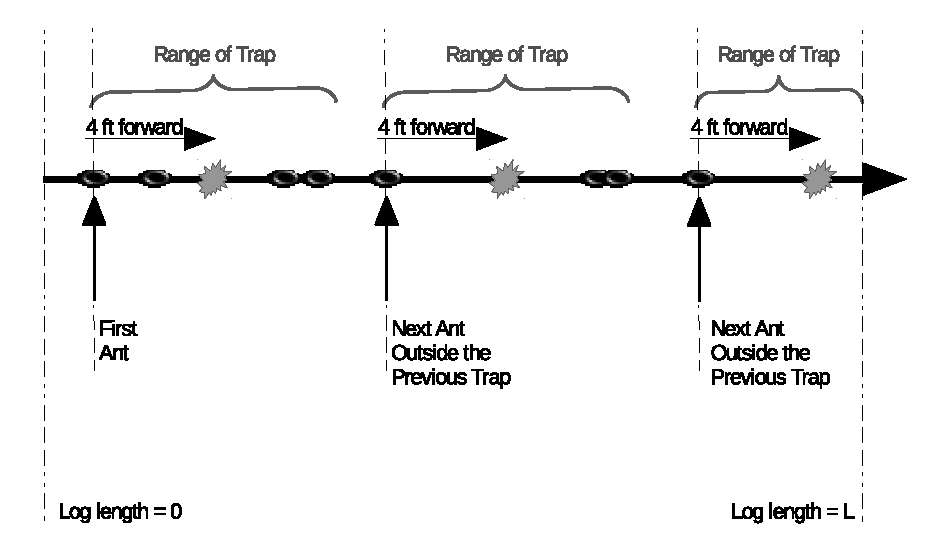
\includegraphics[width=6in]{ants.eps}}
		\caption{$\proc{Ant-Trap}(L,N)$ algorithm starting from left to right}
		\label{fig:ants}
	\end{figure}

	
	This algorithm iterates from the leftmost side of the log and finds ants. Once the first ant is found it places the trap $t_j$, 4 feet forward. In this case all ants in the range of $[t_j-4, t_j+4]$ are all trapped in trap $t_j$. 
	
	To find the next trap, algorithm iterates to find the first ant outside of outside of trap $t_j$. Once found, it places the next trap $t_{j+1}$ 4 feet forward. The algorithm keeps placing traps until all ants are trapped.
	

	   
		
	\begin{codebox}
		\Procname{$\proc{Ant-Trap}(L,N)$}
		
		\li \Comment set $i=1$ to start from the leftmost ant on the log 
		\li $i=1$

		\li \Comment set $j=1$ to start with initializing the first trap 
		\li $j=1$
		
		\li \While $i\leq N$
			\Do	
		\li 	\If $j==1$
				\Do
		\li \Comment if $j=1$ $\rightarrow$ it is the first trap to find $\rightarrow$ find the first ant and place trap 4 feed forward 
		\li 		$t_j=a_i+4$

		\li 	\Else
		\li \Comment if $j \neq 1$ $\rightarrow$ this is not the first trap. To place the next trap, the first ant ouside 
		\li \Comment the previous trap must be found first, and then next trap is placed 4 feed forward.

		\li			\If $a_i>t_j+4$
					\Do
		\li 			$j=j+1$
		\li				$t_j=min(a_i+4,L)$
					\End
				\End
		\li \Comment iterate to next ant
		\li $i=i+1$
			\End

		
	\end{codebox}





	
	
	
	
	
	





































   
\end{enumerate}

\end{document}

